\documentclass{article}
\usepackage{amsmath}
\usepackage{amsfonts}
\usepackage{graphicx}
\usepackage{placeins}
\usepackage{geometry}
\usepackage{minted}
\usepackage{hyperref}

\author{Jaakko Hannikainen - Compilers}
\title{Miniplc, an interpreter for the MiniPL programming language}

\begin{document}
\maketitle

\noindent
\begin{minipage}{0.49\textwidth}
\begin{minted}{text}
var nTimes : int := 0;
print "How many times? ";
read nTimes;
var x : int;
for x in 0..nTimes-1 do
    print x;
    print " : Hello, World!\n";
end for;
assert (x = nTimes);
\end{minted}
\end{minipage}
\begin{minipage}{0.49\textwidth}
\begin{minted}{text}
$ java -jar build/libs/miniplc.jar loopExample.mpl
How many times? 5
0 : Hello, World!
1 : Hello, World!
2 : Hello, World!
3 : Hello, World!
4 : Hello, World!
$
\end{minted}
\end{minipage}

\section{Introduction}
Basic usage:
\begin{minted}{shell}
    ./gradlew jar
    java -jar build/libs/miniplc.jar helloWorld.mpl
\end{minted}

\noindent
Running tests:
\begin{minted}{shell}
    ./gradlew test # normal unit tests
    ./gradlew pitest # unit tests with mutation tests
\end{minted}

\section{Architecture}
The interpreter has a simple multi-pass design, first the program is tokenized,
and then resulting token stream is parsed using a simple grammar. The resulting
tree is then executed.

The tokenizer (fi.jgke.miniplc.tokenizer.Tokenizer) is a simple state machine
tokenizer - As long as the input stream is not empty, the tokenizer parses a
single token from the stream. The tokens are then returned to the Executor
(fi.jgke.miniplc.interpreter.Executor), which gives the resulting stream to the
tree parser, located in the package fi.jgke.miniplc.builder. The parser is
trivially modifiable to enable parsing LL(k) grammars, but in the case of this
language, only LL(1) features are used.

\newpage

The syntax of the language is handled using a simple Java-based DSL, located in
fi.jgke.miniplc.builder.Syntax.

\begin{minted}{Java}
/*
 * <expression> ::= <unaryOperator> <operand>
 *               | <operand> [<binaryOperator> <operand>]
 */
public static Rule expression() {
    return lazy(() -> any(
            rule(ExpressionHandlers::handleNot,
                 Not, operand()),
            rule(ExpressionHandlers::handleOperation,
                 operand(), maybe(operator(), operand()))
    ));
}
\end{minted}

The above example is the parse rules for expressions. The rule states that an
expression is a token stream which either begins with a "not" or any operand.
The tree is then parsed: if the topmost token is "not", then it is taken off
the token stream, and an operand is parsed. Otherwise, an operand is parsed,
and if the token stream follows with an operator, a second operand is also
parsed. If neither of these is true, an exception is thrown. When the parsing
is complete, the token list is passed to the handler, in this case, either
handleNot or handleOperation.

\FloatBarrier
\begin{figure}[ht!]
    \begin{center}
        \makebox[\textwidth]{
            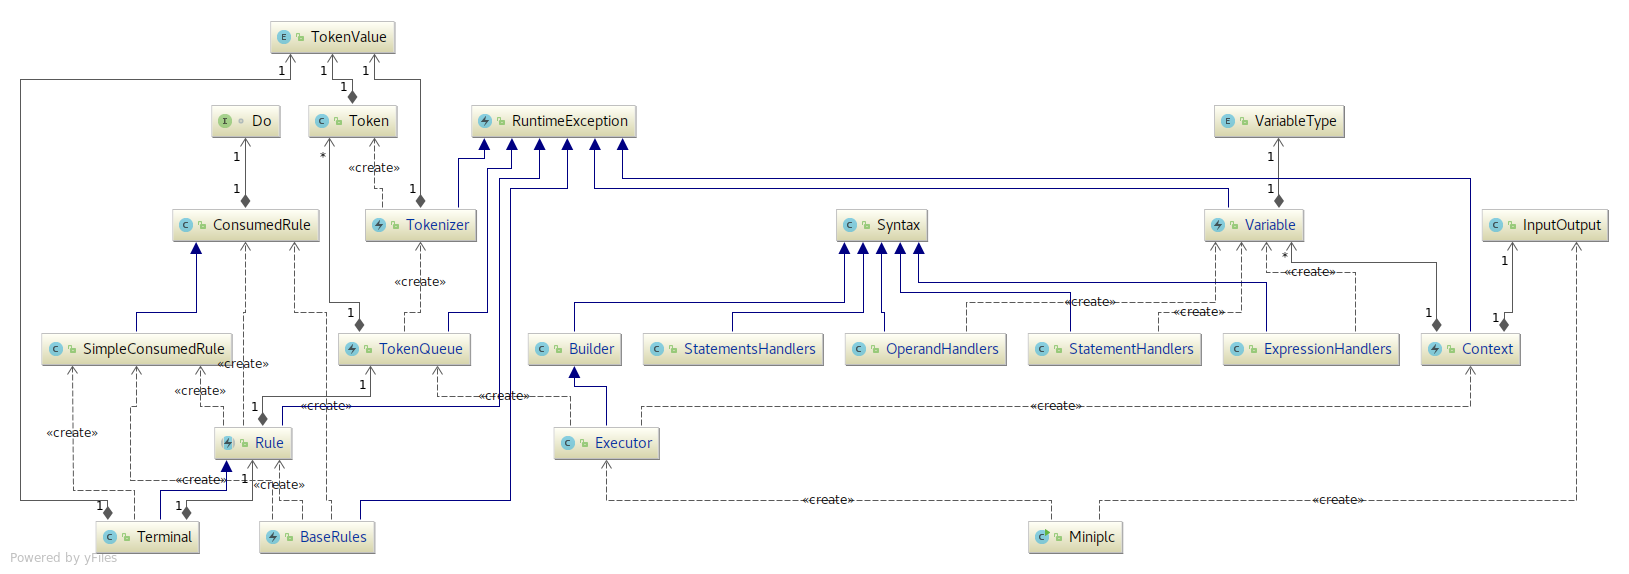
\includegraphics[width=\paperwidth]{diagram}}
    \end{center}
    \caption{Simplified UML diagram, generated using IntelliJ IDEA.}
    \label{fig:uml}
\end{figure}
\FloatBarrier

\section{Testing}
The interpreter has a comprehensive automatic test suite.
\newpage

\section{LL(1) Syntax}

\begin{minted}[mathescape, escapeinside=&&]{text}
 <prog>   ::=  <stmt> ";" <stmts>

 <stmts>  ::=  <stmt> ";" <stmts>
           |   &$\varepsilon$&

 <stmt>   ::=  "var" <var_ident> ":" <type> <maybe_assign>
           |   "for" <var_ident> "in" <expr> ".." <expr> "do"
                  <stmts> "end" "for"
           |   "read" <var_ident>
           |   "print" <expr>
           |   "assert" "(" <expr> ")"
           |   <var_ident> ":=" <expr>

 <maybe_assign> ::= ":=" <expr>
                 |   &$\varepsilon$&

 <expr>   ::= <unary_op> <opnd>
            | <opnd> <maybe_operand>

 <maybe_operand> ::= <binary_op> <opnd>
                  |  &$\varepsilon$&

 <opnd>   ::=  <int>
           |   <string>
           |   <bool>
           |   <var_ident>
           |   "(" expr ")"

 <type>   ::=  "int" | "string" | "bool"
 <var_ident> ::= <ident>

 <reserved keyword> ::=
              "var" | "for" | "end" | "in" | "do" | "read" |
              "print" | "int" | "string" | "bool" | "assert"
\end{minted}

\section{Compiler}
The error messages could use some more work.

The internal representation is given using a DSL, which is parsed to a tree of
so-called "Consumed rules" - which are rules which have consumed tokens.

Error handling is simple - something goes wrong, exceptions are thrown.

\section{Original project definition}

This is a copy of the original project definition located at
\url{https://www.cs.helsinki.fi/u/vihavain/k16/Compilers/project/miniplsyntax\_2016.html}

\subsection{Syntax and semantics of Mini-PL (9.2.2016)}
Mini-PL is a simple programming language designed for pedagogic purposes. The
language is purposely small and is not actually meant for any real programming.
Mini-PL contains few statements, arithmetic expressions, and some IO
primitives. The language uses static typing and has three built-in types
representing primitive values: int, string, and bool. The BNF-style syntax of
Mini-PL is given below, and the following paragraphs informally describe the
semantics of the language.

Mini-PL uses a single global scope for all different kinds of names. All
variables must be declared before use, and each identifier may be declared once
only. If not explicitly initialized, variables are assigned an appropriate
default value.

The Mini-PL read statement can read either an integer value or a single word
(string) from the input stream. Both types of items are whitespace-limited (by
blanks, newlines, etc). Likewise, the print statement can write out either
integers or string values. A Mini-PL program uses default input and output
channels defined by its environment. Additionally, Mini-PL includes an assert
statement that can be used to verify assertions (assumptions) about the state
of the program. An assert statement takes a bool argument. If an assertion
fails (the argument is false) the system prints out a diagnostic message.  The
arithmetic operator symbols '+', '-', '*','/' represent the following
functions:

\begin{minted}{text}
  "+" : (int, int) -> int            // integer addition
  "-" : (int, int) -> int            // integer subtraction
  "*" : (int, int) -> int            // integer multiplication
  "/" : (int, int) -> int            // integer division
\end{minted}
The operator '+' also represents string concatenation (i.e., this operator
symbol is overloaded):

\begin{minted}{text}
  "+" : (string, string) -> string   // string concatenation
\end{minted}
The operators '\&' and '!' represent logical operations:

\begin{minted}{text}
  "\&" : (bool, bool) -> bool         // logical and
  "!" : (bool) -> bool                // logical not
\end{minted}
The operators '=' and b '<' are overloaded to represent the comparisons between
two values of the same type T (int, string, or bool):

\begin{minted}{text}
  "=" : (T, T) -> bool               // equality comparison
  "<" : (T, T) -> bool               // less-than comparison
\end{minted}
A for statement iterates over the consequent values from a specified integer
range. The expressions specifying the beginning and end of the range are
evaluated once only (at the beginning of the for statement). The for control
variable behaves like a constant inside the loop: it cannot be assigned another
value (before exiting the for statement). A control variable needs to be
declared before its use in the for statement (in the global scope). Note that
loop control variables are not declared inside for statements.

\subsection{Context-free grammar for Mini-PL}
The syntax definition is given in so-called Extended Backus-Naur form (EBNF).
In the following Mini-PL grammar, the notation X* means 0, 1, or more
repetitions of the item X. The '|' operator is used to define alternative
constructs. Parentheses may be used to group together a sequence of related
symbols. Brackets ("[" "]") may be used to enclose optional parts (i.e., zero
or one occurrence). Reserved keywords are marked bold (as "var"). Operators,
separators, and other single or multiple character tokens are enclosed within
quotes (as: ".."). Note that nested expressions are always fully parenthesized
to specify the execution order of operations.

\begin{minted}{text}
 <prog>   ::=  <stmts>
 <stmts>  ::=  <stmt> ";" ( <stmt> ";" )*
 <stmt>   ::=  "var" <var_ident> ":" <type> [ ":=" <expr> ]
           |   <var_ident> ":=" <expr>
           |   "for" <var_ident> "in" <expr> ".." <expr> "do"
                  <stmts> "end" "for"
           |   "read" <var_ident>
           |   "print" <expr>
           |   "assert" "(" <expr> ")"

 <expr>   ::=  <opnd> <op> <opnd>
           |   [ <unary_op> ] <opnd>

 <opnd>   ::=  <int>
           |   <string>
           |   <var_ident>
           |   "(" expr ")"

 <type>   ::=  "int" | "string" | "bool"
 <var_ident> ::= <ident>

 <reserved keyword> ::=
              "var" | "for" | "end" | "in" | "do" | "read" |
              "print" | "int" | "string" | "bool" | "assert"
\end{minted}
\subsection{Lexical elements}

In the syntax definition the symbol <ident> stands for an identifier (name). An
identifier is a sequence of letters, digits, and underscores, starting with a
letter. Uppercase letters are distinguished from lowercase.

In the syntax definition the symbol <int> stands for an integer constant
(literal). An integer constant is a sequence of decimal digits. The symbol
<string> stands for a string literal. String literals follow the C-style
convention: any special characters, such as the quote character (") or
backslash (\\), are represented using escape characters (e.g.: \\").

A limited set of operators include (only!) the ones listed below.

\begin{minted}{text}
'+' | '-' | '*' | '/' | '<' | '=' | '\&' | '!'
\end{minted}

In the syntax definition the symbol <op> stands for a binary operator symbol.
There is one unary operator symbol (<unary\_op>): '!', meaning the logical not
operation. The operator symbol '\&' stands for the logical and operation. Note
that in Mini-PL, '=' is the equal operator - not assignment.

The predefined type names (e.g.,"int") are reserved keywords, so they cannot be
used as (arbitrary) identifiers. In a Mini-PL program, a comment may appear
between any two tokens. There are two forms of comments: one starts with "/*",
ends with "*/", can extend over multiple lines, and may be nested. The other
comment alternative begins with "//" and goes only to the end of the line.

\subsection{Sample programs}
\begin{minted}{text}
     var X : int := 4 + (6 * 2);
     print X;

     var nTimes : int := 0;
     print "How many times?";
     read nTimes;
     var x : int;
     for x in 0..nTimes-1 do
         print x;
         print " : Hello, World!\n";
     end for;
     assert (x = nTimes);

     print "Give a number";
     var n : int;
     read n;
     var v : int := 1;
     var i : int;
     for i in 1..n do
         v := v * i;
     end for;
     print "The result is: ";
     print v;
\end{minted}

\end{document}
